\documentclass[onecolumn, compsoc,11pt]{IEEEtran}
\usepackage{enumitem}
\usepackage{etex}
\usepackage{amssymb,amsfonts,amsmath,amsthm}
\usepackage{graphicx}
\usepackage{booktabs}
\usepackage[usenames,x11names, dvipsnames, svgnames]{xcolor}
\usepackage{amsmath,amssymb}
\usepackage{dsfont}
\usepackage{amsfonts}
\usepackage{mathrsfs}
\usepackage{texshade}
\usepackage{hyperref}
\hypersetup{
  colorlinks=true,
  linkcolor=black,
  citecolor=blue,
  filecolor=black,
  urlcolor=DodgerBlue4,
  breaklinks=false,
  % linkbordercolor=red,% hyperlink borders will be red
  % pdfborderstyle={/S/U/W 1}% border style will be underline of width 1pt
}
\usepackage{array}
\usepackage{xr}
\usepackage{verbatim}
\usepackage{multirow}
\usepackage{longtable}
\usepackage{tikz-network}
\usepackage[T1,euler-digits]{eulervm}
\usepackage{times}
% \usepackage{pxfonts}
\usepackage{tikz}
\usepackage{pgfplots}
\usetikzlibrary{shapes,calc,shadows,fadings,arrows,decorations.pathreplacing,automata,positioning}
\usetikzlibrary{external}
\usetikzlibrary{decorations.text}
\usepgfplotslibrary{colorbrewer} 
\usepgfplotslibrary{statistics}

\tikzexternalize[prefix=./Figures/External/]% activate externalization!
\tikzexternaldisable
% \addtolength{\voffset}{.1in}  
\usepackage{geometry}
\geometry{letterpaper, left=.6in,right=.6in,top=.5in,bottom=0.7in}

%\addtolength{\textwidth}{-.1in}    
%\addtolength{\hoffset}{.05in}    
%\addtolength{\textheight}{.1in}    
%\addtolength{\footskip}{0in}    
\usepackage{rotating}
\definecolor{nodecol}{RGB}{240,240,220}
\definecolor{nodeedge}{RGB}{240,240,225}
\definecolor{edgecol}{RGB}{130,130,130}
\tikzset{%
  fshadow/.style={      preaction={
      fill=black,opacity=.3,
      path fading=circle with fuzzy edge 20 percent,
      transform canvas={xshift=1mm,yshift=-1mm}
    }} 
}
\usetikzlibrary{pgfplots.dateplot}
\usetikzlibrary{patterns}
\usetikzlibrary{decorations.markings}
\usepackage{fancyhdr}
\usepackage{mathtools}
\usepackage{datetime}
\usepackage{comment}
%% ## Equation Space Control---------------------------
\def\EQSP{3pt}
\newcommand{\mltlne}[2][\EQSP]{\begingroup\setlength\abovedisplayskip{#1}\setlength\belowdisplayskip{#1}\begin{equation}\begin{multlined} #2 \end{multlined}\end{equation}\endgroup\noindent}
\newcommand{\cgather}[2][\EQSP]{\begingroup\setlength\abovedisplayskip{#1}\setlength\belowdisplayskip{#1}\begin{gather} #2 \end{gather}\endgroup\noindent}
\newcommand{\cgathers}[2][\EQSP]{\begingroup\setlength\abovedisplayskip{#1}\setlength\belowdisplayskip{#1}\begin{gather*} #2 \end{gather*}\endgroup\noindent}
\newcommand{\calign}[2][\EQSP]{\begingroup\setlength\abovedisplayskip{#1}\setlength\belowdisplayskip{#1}\begin{align} #2 \end{align}\endgroup\noindent}
\newcommand{\caligns}[2][\EQSP]{\begingroup\setlength\abovedisplayskip{#1}\setlength\belowdisplayskip{#1}\begin{align*} #2 \end{align*}\endgroup\noindent}
\newcommand{\mnp}[2]{\begin{minipage}{#1}#2\end{minipage}} 
%% COLOR DEFS------------------------------------------
\newtheorem{thm}{Theorem}
\newtheorem{cor}{Corollary}
\newtheorem{lem}{Lemma}
\newtheorem{prop}{Proposition}
\newtheorem{defn}{Definition}
\newtheorem{exmpl}{Example}
\newtheorem{rem}{Remark}
\newtheorem{notn}{Notation}
%% ------------PROOF INCLUSION -----------------
\def\NOPROOF{Proof omitted.}
\newif\ifproof
\prooffalse % or \draftfalse
\newcommand{\Proof}[1]{
  \ifproof
  \begin{IEEEproof}
    #1\end{IEEEproof}
  \else
  \NOPROOF
  \fi
}
%% ------------ -----------------
\newcommand{\DETAILS}[1]{#1}
%% ------------ -----------------
% color commands------------------------
\newcommand{\etal}{\textit{et} \mspace{3mu} \textit{al.}}
% \renewcommand{\algorithmiccomment}[1]{$/** $ #1 $ **/$}
\newcommand{\vect}[1]{\textbf{\textit{#1}}}
\newcommand{\figfont}{\fontsize{8}{8}\selectfont\strut}
\newcommand{\hlt}{ \bf \sffamily \itshape\color[rgb]{.1,.2,.45}}
\newcommand{\pitilde}{\widetilde{\pi}}
\newcommand{\Pitilde}{\widetilde{\Pi}}
\newcommand{\bvec}{\vartheta}
\newcommand{\algo}{\textrm{\bf\texttt{GenESeSS}}\xspace}
\newcommand{\xalgo}{\textrm{\bf\texttt{xGenESeSS}}\xspace}
\newcommand{\FNTST}{\bf }
\newcommand{\FNTED}{\color{darkgray} \scriptsize $\phantom{.}$}
\renewcommand{\baselinestretch}{.9}
\newcommand{\sync}{\otimes}
\newcommand{\psync}{\hspace{3pt}\overrightarrow{\hspace{-3pt}\sync}}
% \newcommand{\psync}{\raisebox{-4pt}{\begin{tikzpicture}\node[anchor=south] (A) {$\sync$};
%   \draw [->,>=stealth] ([yshift=-2pt, xshift=2pt]A.north west) -- ([yshift=-2pt]A.north east); %\end{tikzpicture}}}
\newcommand{\base}[1]{\llbracket #1 \rrbracket}
\newcommand{\nst}{\textrm{\sffamily\textsc{Numstates}}}
\newcommand{\HA}{\boldsymbol{\mathds{H}}}
\newcommand{\eqp}{ \vartheta }
\newcommand{\entropy}[1]{\boldsymbol{h}\left ( #1 \right )}
\newcommand{\norm}[1]{\left\lVert #1 \right\rVert}%
\newcommand{\abs}[1]{\left\lvert #1 \right\rvert}%
\newcommand{\absB}[1]{\big\lvert #1 \big\rvert}%
% #############################################################
% #############################################################
% PREAMBLE ####################################################
% #############################################################
% #############################################################
% \usepackage{pnastwoF}      
\DeclareMathOperator*{\argmax}{argmax}
\DeclareMathOperator*{\argmin}{arg\,min}
\DeclareMathOperator*{\expect}{\mathbf{E}}
\DeclareMathOperator*{\var}{\mathbf{Var}}

\newcommand{\ND}{ \mathcal{N}  }
\usepackage[linesnumbered,ruled,vlined,noend]{algorithm2e}
\newcommand{\captionN}[1]{\caption{\color{darkgray} \sffamily \fontsize{9}{10}\selectfont #1  }}
\newcommand{\btl}{\ \textbf{\small\sffamily bits/letter}}
%\usepackage{txfonts}
%%% \usepackage{ccfonts}
%%% save defaults
%\renewcommand{\rmdefault}{phv} % Arial
%\renewcommand{\sfdefault}{phv} % Arial
%\edef\keptrmdefault{\rmdefault}
%\edef\keptsfdefault{\sfdefault}
%\edef\keptttdefault{\ttdefault}

% \usepackage{kerkis}
%\usepackage[OT1]{fontenc}
%\usepackage{concmath}
% \usepackage[T1]{eulervm} 
% \usepackage[OT1]{fontenc}
%%% restore defaults
%\edef\rmdefault{\keptrmdefault}
%\edef\sfdefault{\keptsfdefault}
%\edef\ttdefault{\keptttdefault}
\tikzexternalenable
% ##########################################################
\tikzfading[name=fade out,
inner color=transparent!0,
outer color=transparent!100]
% ###################################
\newcommand{\xtitaut}[2]{
  \noindent\mnp{\textwidth}{
    \mnp{\textwidth}{\raggedright\Huge \bf \sffamily #1}

    \vskip 1em

    {\bf \sffamily #2}
  }
  \vskip 2em
}
% ###################################
% ###################################
\tikzset{wiggle/.style={decorate, decoration={random steps, amplitude=10pt}}}
\usetikzlibrary{decorations.pathmorphing}
\pgfdeclaredecoration{Snake}{initial}
{
  \state{initial}[switch if less than=+.625\pgfdecorationsegmentlength to final,
  width=+.3125\pgfdecorationsegmentlength,
  next state=down]{
    \pgfpathmoveto{\pgfqpoint{0pt}{\pgfdecorationsegmentamplitude}}
  }
  \state{down}[switch if less than=+.8125\pgfdecorationsegmentlength to end down,
  width=+.5\pgfdecorationsegmentlength,
  next state=up]{
    \pgfpathcosine{\pgfqpoint{.25\pgfdecorationsegmentlength}{-1\pgfdecorationsegmentamplitude}}
    \pgfpathsine{\pgfqpoint{.25\pgfdecorationsegmentlength}{-1\pgfdecorationsegmentamplitude}}
  }
  \state{up}[switch if less than=+.8125\pgfdecorationsegmentlength to end up,
  width=+.5\pgfdecorationsegmentlength,
  next state=down]{
    \pgfpathcosine{\pgfqpoint{.25\pgfdecorationsegmentlength}{\pgfdecorationsegmentamplitude}}
    \pgfpathsine{\pgfqpoint{.25\pgfdecorationsegmentlength}{\pgfdecorationsegmentamplitude}}
  }
  \state{end down}[width=+.3125\pgfdecorationsegmentlength,
  next state=final]{
    \pgfpathcosine{\pgfqpoint{.15625\pgfdecorationsegmentlength}{-.5\pgfdecorationsegmentamplitude}}
    \pgfpathsine{\pgfqpoint{.15625\pgfdecorationsegmentlength}{-.5\pgfdecorationsegmentamplitude}}
  }
  \state{end up}[width=+.3125\pgfdecorationsegmentlength,
  next state=final]{
    \pgfpathcosine{\pgfqpoint{.15625\pgfdecorationsegmentlength}{.5\pgfdecorationsegmentamplitude}}
    \pgfpathsine{\pgfqpoint{.15625\pgfdecorationsegmentlength}{.5\pgfdecorationsegmentamplitude}}
  }
  \state{final}{\pgfpathlineto{\pgfpointdecoratedpathlast}}
}
% ###################################
% ###################################
\newcolumntype{L}[1]{>{\rule{0pt}{2ex}\raggedright\let\newline\\\arraybackslash\hspace{0pt}}m{#1}}
\newcolumntype{C}[1]{>{\rule{0pt}{2ex}\centering\let\newline\\\arraybackslash\hspace{0pt}}m{#1}}
\newcolumntype{R}[1]{>{\rule{0pt}{2ex}\raggedleft\let\newline\\\arraybackslash\hspace{0pt}}m{#1}}



% ################################################
% ################################################
% ################################################
% ################################################
\def\DISCLOSURE#1{\def\disclosure{#1}}
\DISCLOSURE{\raisebox{15pt}{$\phantom{XxxX}$This sheet contains proprietary information 
    not to be released to third parties except for the explicit purpose of evaluation.}
}
% ####################################
\newcommand{\set}[1]{\left\{ #1 \right\}}
\newcommand{\paren}[1]{\left( #1 \right)}
\newcommand{\bracket}[1]{\left[ #1 \right]}
% \newcommand{\norm}[1]{\left\Vert #1 \right\Vert}
\newcommand{\nrm}[1]{\left\llbracket{#1}\right\rrbracket}
\newcommand{\parenBar}[2]{\paren{#1\,{\left\Vert\,#2\right.}}}
\newcommand{\parenBarl}[2]{\paren{\left.#1\,\right\Vert\,#2}}
\newcommand{\ie}{$i.e.$\xspace}
\newcommand{\addcitation}{\textcolor{black!50!red}{\textbf{ADD CITATION}}}
\newcommand{\subtochange}[1]{{\color{black!50!green}{#1}}}
\newcommand{\tobecompleted}{{\color{black!50!red}TO BE COMPLETED.}}


\newcommand{\pIn}{\mathscr{P}_{\textrm{in}}}
\newcommand{\pOut}{\mathscr{P}_{\textrm{out}}}
\newcommand{\aIn}[1][\Sigma]{#1_{\textrm{in}}}
\newcommand{\aOut}[1][\Sigma]{#1_{\textrm{out}}}
\newcommand{\xin}[1]{#1_{\textrm{in}}}
\newcommand{\xout}[1]{#1_{\textrm{out}}}

\newcommand{\R}{\mathbb{R}} % Set of real numbers
\newcommand{\F}[1][]{\mathcal{F}_{#1}}
\newcommand{\SR}{\mathcal{S}} % Semiring of sets
\newcommand{\RR}{\mathcal{R}} % Ring of sets
\newcommand{\N}{\mathbb{N}} % Set of natural numbers (0 included)


\newcommand{\Pp}[1][n]{\mathscr{P}^+_{#1}}
\renewcommand{\entropy}[1]{\boldsymbol{h}\left ( #1 \right )}



\makeatletter
\pgfdeclarepatternformonly[\hatchdistance,\hatchthickness]{flexible hatch}
{\pgfqpoint{0pt}{0pt}}
{\pgfqpoint{\hatchdistance}{\hatchdistance}}
{\pgfpoint{\hatchdistance-1pt}{\hatchdistance-1pt}}%
{
  \pgfsetcolor{\tikz@pattern@color}
  \pgfsetlinewidth{\hatchthickness}
  \pgfpathmoveto{\pgfqpoint{0pt}{0pt}}
  \pgfpathlineto{\pgfqpoint{\hatchdistance}{\hatchdistance}}
  \pgfusepath{stroke}
}
\makeatother

\pgfdeclarepatternformonly{north east lines wide}%
{\pgfqpoint{-1pt}{-1pt}}%
{\pgfqpoint{10pt}{10pt}}%
{\pgfqpoint{9pt}{9pt}}%
{
  \pgfsetlinewidth{0.7pt}
  \pgfpathmoveto{\pgfqpoint{0pt}{0pt}}
  \pgfpathlineto{\pgfqpoint{9.1pt}{9.1pt}}
  \pgfusepath{stroke}
}

\pgfdeclarepatternformonly{north west lines wide}%
{\pgfqpoint{-1pt}{-1pt}}%
{\pgfqpoint{10pt}{10pt}}%
{\pgfqpoint{9pt}{9pt}}%
{
  \pgfsetlinewidth{0.7pt}
  \pgfpathmoveto{\pgfqpoint{0pt}{9pt}}
  \pgfpathlineto{\pgfqpoint{9.1pt}{-0.1pt}}
  \pgfusepath{stroke}
}
\makeatletter

\pgfdeclarepatternformonly[\hatchdistance,\hatchthickness]{flexible hatchB}
{\pgfqpoint{0pt}{\hatchdistance}}
{\pgfqpoint{\hatchdistance}{0pt}}
{\pgfpoint{1pt}{\hatchdistance-1pt}}%
{
  \pgfsetcolor{\tikz@pattern@color}
  \pgfsetlinewidth{\hatchthickness}
  \pgfpathmoveto{\pgfqpoint{0pt}{\hatchdistance}}
  \pgfpathlineto{\pgfqpoint{\hatchdistance}{0pt}}
  \pgfusepath{stroke}
}    \makeatother


\def\TPR{\textrm{TPR}\xspace}
\def\TNR{\textrm{TNR}\xspace}
\def\FPR{\textrm{FPR}\xspace}
\def\PPV{\textrm{PPV}\xspace}

\usetikzlibrary{arrows.meta}
\usetikzlibrary{decorations.pathreplacing,shapes.misc}
\usepgfplotslibrary{fillbetween}
%usepackage{tikz-network}
\usetikzlibrary{shapes.geometric}
\usetikzlibrary{math}
\usepgfplotslibrary{colorbrewer} 

\usepackage{textcomp}
\usepackage{colortbl}
\usepackage{array}
\usepackage{courier} 
\usepackage{wrapfig}
\usepackage{pifont}
\usetikzlibrary{chains,backgrounds}
\usetikzlibrary{intersections}
\usetikzlibrary{pgfplots.groupplots}
\usepgfplotslibrary{fillbetween} 
\usetikzlibrary{arrows.meta}
\usepackage{pgfplotstable}
\usepackage[super,compress,sort,comma]{natbib}
%\usepackage{natbib}
\usepackage{setspace}
\usetikzlibrary{math}
\usetikzlibrary{matrix}
\usepackage{xstring}
\usepackage{xspace}
\usepackage{flushend}
\makeatletter
\renewcommand\section{\@startsection {section}{1}{\z@}%
  {-2ex \@plus -1ex \@minus -.2ex}%
  {1ex \@plus.1ex}%
  {\Large\bfseries\scshape}}
\renewcommand\subsection{\@startsection {subsection}{1}{\z@}%
  {-2ex \@plus -.25ex \@minus -.2ex}%
  {0.1ex \@plus.0ex}%
  {\fontsize{11}{10}\selectfont\bfseries\sffamily\color{black}}}
\renewcommand\subsubsection{\@startsection {subsubsection}{1}{\z@}%
  {0ex \@plus -.5ex \@minus -.2ex}%
  {0.0ex \@plus.5ex}%
  {\bfseries\itshape\sffamily\color{darkgray}}}
\renewcommand\paragraph{\@startsection {paragraph}{1}{\z@}%
  {-.2ex \@plus -.5ex \@minus -.2ex}%
  {0.0ex \@plus.5ex}%
  {\fontsize{9}{9}\selectfont\itshape\sffamily\color{darkgray}}}
       
%\renewcommand{\thesubsection}{\thesection.\arabic{subsection}}
\renewcommand{\thesubsectiondis}{\arabic{subsection}.}
\renewcommand{\thesectiondis}{\arabic{section}.}
\renewcommand{\thesection}{\arabic{section}}

\renewcommand{\thetable}{\arabic{table}}

\makeatother
\makeatletter
\pgfdeclareradialshading[tikz@ball]{ball}{\pgfqpoint{-10bp}{10bp}}{%
  color(0bp)=(tikz@ball!30!white);
  color(9bp)=(tikz@ball!75!white);
  color(18bp)=(tikz@ball!90!black);
  color(25bp)=(tikz@ball!70!black);
  color(50bp)=(black)}
\makeatother
%\newcommand{\tball}[1][CadetBlue4]{${\color{#1}\Large\boldsymbol{\blacksquare}}$}
\renewcommand{\baselinestretch}{1}
%\renewcommand{\captionN}[1]{\caption{\color{CadetBlue4!50!black} \sffamily \fontsize{9}{10}\selectfont #1  }}
\tikzexternaldisable 
\parskip=6pt
\parindent=0pt
%\newcommand{\Mark}[1]{\textsuperscript{#1}}
\pagestyle{fancy}

\newcounter{Dcounter}
\setcounter{Dcounter}{1}
\newcommand{\DQS}[1]{\marginpar{\tikzexternaldisable \tikz{\node[rounded corners=5pt,draw=none,thick,fill=black!10,font=\sffamily\fontsize{7}{8}\selectfont] {\mnp{.45in} {\color{Red3}\raggedright  \#\theDcounter.~#1}}; }}\stepcounter{Dcounter}\xspace}

\newcommand{\qn}[1][i]{\Phi_{#1}}
\newcommand{\D}[1][i]{\mathscr{D}\left ( {\Sigma_#1} \right ) }
\newcommand{\Dx}{\mathscr{D}}
\def\J{\mathds{J}}
\def\M{\omega}
\def\N{\mathds{N}}
\newcommand{\cp}[1][P]{\langle #1 \rangle}
\newcommand{\mem}[1]{\M_{#1}}


\makeatletter
\newcommand\transformxdimension[1]{
    \pgfmathparse{((#1/\pgfplots@x@veclength)+\pgfplots@data@scale@trafo@SHIFT@x)/10^\pgfplots@data@scale@trafo@EXPONENT@x}
}
\newcommand\transformydimension[1]{
    \pgfmathparse{((#1/\pgfplots@y@veclength)+\pgfplots@data@scale@trafo@SHIFT@y)/10^\pgfplots@data@scale@trafo@EXPONENT@y}
}
\makeatother

\parskip=6pt
\parindent=0pt


\pgfplotsset{
    discard if/.style 2 args={
        x filter/.code={
            \edef\tempa{\thisrow{#1}}
            \edef\tempb{#2}
            \ifx\tempa\tempb
                \def\pgfmathresult{inf}
            \fi
        }
    },
    discard if not/.style 2 args={
        x filter/.code={
            \edef\tempa{\thisrow{#1}}
            \edef\tempb{#2}
            \ifx\tempa\tempb
            \else
                \def\pgfmathresult{inf}
            \fi
        }
    }
  }

  %\newcommand{\HLT}[2][Red1]{{\color{#1}#2}}

 % \def\commatonone{\expandafter\zappointzerozero
%    \romannumeral`\^^@}
%\def\zappointzerozero#1.00{\zapcomma#1,!}
%\def\zapcomma#1,#2{#1\ifx!#2\else#2\expandafter\zapcomma\fi}
\def\commatononei#1,{#1}
\def\commatononej#1,#2,{#1#2}
\def\commatonone#1{\expandafter\commatononei#1}
\def\commatononeT#1{\expandafter\commatononej#1}
\newcommand{\Sum} [2] {#1 + #2 = \the\numexpr #1 + #2 \relax \\}


\usepackage{sistyle}
\SIthousandsep{,}

\makeatletter
\newcommand{\limitpages}[1]{
  \gdef\maxpages{#1}%
  \ifx\latex@outputpage\@undefined\relax%
  \global\let\latex@outputpage\@outputpage%
  \fi%
  \gdef\@outputpage{%
    \ifnum\value{page}>\maxpages\relax%
    % Do not output the page
    \else%
    \latex@outputpage%
    \fi%
  }%
}
\makeatother
\newcommand{\note}[1]{{ \itshape \footnotesize \color{Red1}$\medbullet$~ #1}}









\renewcommand{\thesectiondis}{\arabic{section}.}
\renewcommand{\thesubsectiondis}{\Alph{subsection}.}

\makeatletter
\renewcommand\section{\@startsection {section}{1}{\z@}%
  {-1pt \@plus -30ex \@minus 20ex}%
  {.1pt}%
  {\large\bfseries\scshape}}
\renewcommand\subsection{\@startsection {subsection}{2}{\z@}%
  {0ex \@plus -1.75ex \@minus -1.2ex}%
  {0ex \@plus.0ex}%
  {\fontsize{11}{11}\selectfont\bfseries\sffamily\color{black}}}
\renewcommand\subsubsection{\@startsection {section}{1}{\z@}%
  {-.1ex \@plus -.5ex \@minus -.2ex}%
  {0.0ex \@plus.5ex}%
  {\bfseries\sffamily\color{Red4}}}
\renewcommand\paragraph{\@startsection {section}{1}{\z@}%
  {-.1ex \@plus -.5ex \@minus -.2ex}%
  {0.0ex \@plus.5ex}%
  {\fontsize{11}{10}\selectfont\bfseries\itshape\sffamily\color{black}}}
\makeatother


\makeatletter
\pgfdeclareradialshading[tikz@ball]{ball}{\pgfqpoint{-10bp}{10bp}}{%
  color(0bp)=(tikz@ball!30!white);
  color(9bp)=(tikz@ball!75!white);
  color(18bp)=(tikz@ball!90!black);
  color(25bp)=(tikz@ball!70!black);
  color(50bp)=(black)}
\makeatother
\newcommand{\tball}{${\color{CadetBlue3}\Large\boldsymbol{\blacksquare}}$}
\renewcommand{\baselinestretch}{.87}
\newcommand{\VSP}{\vspace{-2pt}}
\renewcommand{\captionN}[1]{\caption{\color{black} \sffamily \fontsize{9}{10}\selectfont #1  }}




\newcommand*{\doi}[1]{\href{http://dx.doi.org/#1}{doi: #1}}
\renewcommand{\IEEEbibitemsep}{20pt plus 2pt}
\makeatletter
\IEEEtriggercmd{\reset@font\normalfont\fontsize{11}{14}\selectfont}
\makeatother
\IEEEtriggeratref{1}
\newlength{\bibitemsep}\setlength{\bibitemsep}{.2\baselineskip plus .05\baselineskip minus .05\baselineskip}
\newlength{\bibparskip}\setlength{\bibparskip}{0pt}
\let\oldthebibliography\thebibliography
\renewcommand\thebibliography[1]{%
  \oldthebibliography{#1}%
  \setlength{\parskip}{\bibitemsep}%
  \setlength{\itemsep}{\bibparskip}%
}
\setlength{\bibitemsep}{.3\baselineskip plus .05\baselineskip minus .05\baselineskip} 
% \usepackage{cite}
\usepackage{textcomp}
\usepackage{colortbl}
\usepackage{subfigure}
\usepackage{array}
\usepackage{courier}
\usepackage{setspace} 
\usepackage{wrapfig} 
\usepackage{calligra}
\usepackage{ulem}
\usepackage{multirow}
\renewcommand{\IEEEbibitemsep}{20pt plus 2pt}
\makeatletter
\IEEEtriggercmd{\reset@font\normalfont\fontsize{11}{14}\selectfont}
\makeatother
\IEEEtriggeratref{1}
\newlength{\bibitemsep}\setlength{\bibitemsep}{.2\baselineskip plus .05\baselineskip minus .05\baselineskip}
\newlength{\bibparskip}\setlength{\bibparskip}{0pt}
\let\oldthebibliography\thebibliography
\renewcommand\thebibliography[1]{%
  \oldthebibliography{#1}%
  \setlength{\parskip}{\bibitemsep}%
  \setlength{\itemsep}{\bibparskip}%
}
\setlength{\bibitemsep}{.3\baselineskip plus .05\baselineskip minus .05\baselineskip}

\usetikzlibrary{chains,backgrounds}
\usetikzlibrary{intersections}
% \usepackage[super]{cite} 
% \makeatletter \renewcommand{\@citess}[1]{\raisebox{1pt}{\textsuperscript{[#1]}}} \makeatother
\usepackage{xstring}
\usepackage{wasysym}
\usepackage[misc]{ifsym}
\renewcommand{\thesectiondis}{\arabic{section}.}
\renewcommand{\thesubsectiondis}{\Alph{subsection}.}

\makeatletter
\renewcommand\section{\@startsection {section}{1}{\z@}%
  {-1pt \@plus -30ex \@minus 20ex}%
  {.1pt}%
  {\large\bfseries\scshape}}
\renewcommand\subsection{\@startsection {subsection}{2}{\z@}%
  {0ex \@plus -1.75ex \@minus -1.2ex}%
  {0ex \@plus.0ex}%
  {\fontsize{11}{11}\selectfont\bfseries\sffamily\color{black}}}
\renewcommand\subsubsection{\@startsection {section}{1}{\z@}%
  {-1.5ex \@plus -.5ex \@minus -.2ex}%
  {0.0ex \@plus.5ex}%
  {\fontsize{9}{9}\selectfont\bfseries\sffamily\color{Red4}}}
\renewcommand\paragraph{\@startsection {section}{1}{\z@}%
  {-.1ex \@plus -.5ex \@minus -.2ex}%
  {0.0ex \@plus.5ex}%
  {\fontsize{11}{10}\selectfont\bfseries\itshape\sffamily\color{black}}}
\makeatother


\makeatletter
\pgfdeclareradialshading[tikz@ball]{ball}{\pgfqpoint{-10bp}{10bp}}{%
  color(0bp)=(tikz@ball!30!white);
  color(9bp)=(tikz@ball!75!white);
  color(18bp)=(tikz@ball!90!black);
  color(25bp)=(tikz@ball!70!black);
  color(50bp)=(black)}
\makeatother
\newcommand{\tball}{${\color{CadetBlue3}\Large\boldsymbol{\blacksquare}}$}
\renewcommand{\baselinestretch}{.94}
\newcommand{\VSP}{\vspace{-2pt}}
\renewcommand{\captionN}[1]{\caption{\color{black} \sffamily \fontsize{9}{10}\selectfont #1  }}
\tikzexternaldisable 
\parskip=4pt
\parindent=0pt
\newcommand{\Mark}[1]{\textsuperscript{#1}}
\lhead{}
\pagestyle{fancy}
\def\COLA{black}
% ###################################
\cfoot{\bf\sffamily \scriptsize \color{Maroon!50} I. Chattopadhyay, Department of Medicine, University of Chicago}
\cfoot{}
\rhead{}
% \rhead{\bf\sffamily \scriptsize \color{DodgerBlue4!50} DARPA Young Faculty Award 2017}
% \rhead{\scriptsize\bf\sffamily \href{zed.UChicago.edu}{zed.UChicago.edu}}
% \rfoot{\scriptsize\bf\sffamily\thepage}
\newcommand{\partxt}{\bf\sffamily\itshape}
% ############################################################
\newif\iftikzX
\tikzXtrue
\tikzXfalse

\newcommand\guline{\bgroup\markoverwith
  {\textcolor{black!30}{\rule[-0.45ex]{2pt}{0.4pt}}}\ULon}
\newcommand\hilit[1]{\textcolor{Red1}{#1}}
\newcommand\hilitx[1]{\guline{#1}}
% ############################################################
\addtolength{\voffset}{.1in}
\addtolength{\textwidth}{-.085in}
\addtolength{\hoffset}{.0425in}
\def\PROG{Mallinckrodt\xspace}
\def\ZERO{ACoR\xspace}
\def\COLWA{\XCOLA!40}
\def\COLWB{\XCOLD!20}
\def\COLWC{\XCOLA!40}
\def\COLWD{\XCOLD!20}
\def\COLWE{\XCOLA!40}
\def\COLWF{\XCOLD!20}
% ############################################################
\def\treatment{positive\xspace}
\def\TITLE{A pharmacogenomic hypothesis for reducing the population risk of autism via potential off-label non-contra-indicated use of a common SSRI agent in pregnant women}
\def\TITLE{A pharmacogenomic hypothesis for reducing   risk of autism}
\def\TOTALCOSTSAMPLES{$\$1875 \times 7 = \$13,125$}
\def\PINAME{Ishanu Chattopadhyay}
\def\PIINST{University of Chicago}
\def\PIEMAIL{\url{ishanu@uchicago.edu}}

\def\SIMONDATA{SSC proband \& matched designated sibling ($672$ samples)}

\def\acor{ACoR\xspace}

\newcommand{\HDR}{
\begin{tabular}{|L{.3\textwidth} | L{.32\textwidth} | L{.3\textwidth} | }\hline
  Principal investigator Name: \bf \PINAME & Principal Investigator Institution: \bf \PIINST & Principal Investigator  email: \PIEMAIL \\\hline
  \multicolumn{2}{|C{.62\textwidth}|}{\hspace{-15pt} \mnp{.63\textwidth}{\vskip .45em Project Title\\ \bf \TITLE \\\vspace{-8pt} }} &  {\mnp{.3\textwidth}{\vskip .3em Project Type: \\ \bf Pilot}} \\\hline
  \multicolumn{3}{|C{.92\textwidth}|}{ \hspace{-40pt} \mnp{.93\textwidth}{\vskip .6em Data requested from Simons Collection:  \SIMONDATA \\ \vspace{-8pt}}} \\\hline
  \multicolumn{2}{|C{.62\textwidth}|}{\hspace{-15pt} \mnp{.63\textwidth}{Total Estimated Cost for Samples (Price List)}}& \TOTALCOSTSAMPLES\\\hline
\end{tabular}
\vskip .5em
}


\begin{document} 

\limitpages{1}

\begin{tabular}{|L{.3\textwidth} | L{.32\textwidth} | L{.3\textwidth} | }\hline
  Principal investigator Name: \bf \PINAME & Principal Investigator Institution: \bf \PIINST & Principal Investigator  email: \PIEMAIL \\\hline
  \multicolumn{2}{|C{.62\textwidth}|}{\hspace{-15pt} \mnp{.63\textwidth}{\vskip .45em Project Title\\ \bf \TITLE \\\vspace{-8pt} }} &  {\mnp{.3\textwidth}{\vskip .3em Project Type: \\ \bf Pilot}} \\\hline
  \multicolumn{3}{|C{.92\textwidth}|}{ \hspace{-40pt} \mnp{.93\textwidth}{\vskip .6em Data requested from a Simons Collection:  \SIMONDATA \\ \vspace{-8pt}}} \\\hline
  \multicolumn{2}{|C{.62\textwidth}|}{\hspace{-15pt} \mnp{.63\textwidth}{Total Estimated Cost for Samples (Price List)}}& \TOTALCOSTSAMPLES\\\hline
\end{tabular}

\vskip .5em


% The Specific Aims Page should not exceed one (1) page of single-spaced, size 11 text, 0.5 margins. This should be a summary of the proposed project focused on the research aims of the project, including a concise rationale for the hypothesis, description of preliminary data and experimental approach, and impact on autism research. 


\section*{Specific Aims}
% \vspace{-5pt}

\lfoot{\thepage \\ Project Summary}
% Despite increasing prevalence, the
While detailed etiology of Autism Spectrum Disorder (ASD) is  unclear~\cite{hyman2020identification,nihasd,bolte2019contribution}, % It has become increasingly clear that  genetic predisposition and environmental effects leading to dysregulation of immune pathways increase risk~\cite{gzielo2021astroglia,pmid30971960,pmid30941018,pmid29691724,pmid29307081,pmid27351598,pmid26793298,pmid30095240,pmid25681541,hyman2020identification}.
% In particular,
 a combination of genetic and environmental factors including xenobiotic exposure  during early % stages of
neurodevelopment % when the immature brain is extremely vulnerable,
are implicated as important risk factors in ASD pathogenesis~\cite{bolte2019contribution,santos2022role}. In this pilot, we  plan to validate % and extend
our preliminary results that may clarify ASD pathobiology of a  subset of non-syndromic cases, defined by specific prescription drugs taken by mothers during pregnancy,  and possibly offer new interventional insights to reduce population risk of disease onset. %Genetic burden modulated by environmental triggers has been implicated in triggering the onset of autism~\cite{bolte2019contribution,santos2022role}, and we offer hypotheses that might clarify the mechanism of onset for some cases.
% and investigate the possibility of operationalizing

\textbf{Hypotheses:} This pilot is centered around  the  hypotheses: 1) Anomalous induction of cytochrome P450 enzyme 2D6 in the fetal brain during early development increases the risk of disease onset,  2) Pre and post-natal pharmacological  mechanism-based-inhibition (MBI) of CYP2D6, especially via off-target effect of the SSRI paroxetine,   can significantly and substantially reduce risk, and 3)  up-regulating Brain-Derived Neurotrophic Factor (BDNF) during pregnancy ($e.g.$ by taking SSRI sertraline) significantly increase risk. Importantly, these hypotheses do not replace the complex genetic burden  implicated in autism etiology, but suggests that specific modes of the xenobiotic response  pathways  might have an important but hitherto under-appreciated role in disease onset, and selective and timely down-regulation of these responses may reduce the onset risk. 

\textbf{Overall Rationale:} Environmental triggers can induce  xenobiotic response via the P450 pathways. It is known that some xenobiotic stimuli can reach the fetus, which can then induce 2D6 activation. Anomalous activation of the 2D6 enzyme may interfere with  brain development, perhaps via impacting the developing glial system~\cite{gzielo2021astroglia,kuban2021cytochrome}. Pharmacological inhibition of the 2D6 pathway reduces the odds of such  activation, thereby reducing the population risk for autism. Certain drug(s) for which we find a population-level protective effect in our preliminary studies $e.g.$ paroxetine~\cite{brosen1998differences},  are known to cross the placenta~\cite{brosen1998differences} and have the desired off-target 2D6 inhibition. Such inhibition may be induced when the mother is exposed to them during pregnancy promoting normal fetal development. On the other hand, some SSRIs which up-regulate BDNF $e.g.$ sertraline~\cite{brosen1998differences} (off-target effect) might  interfere with  neurodevelopment~\cite{kasarpalkar2014brain}; consistent with our observed elevated population risk. 

\textbf{Preliminary Data:} Using IBM Marketscan administrative database, we associated the history of medical encounters of pregnant women with the eventual ASD status of their children (n=184,438), and found significant and substantial protective as well as risk-increasing signals for specific drugs, that merit detailed investigation. %Here, we plan  to further evaluate these effects  both retrospectively and  prospectively in this effort. %Our preliminary study on large national familial-linked Electronic Health Record dataset (n=184,438) provides retrospective evidence that some prescribed SSRIs have a substantial and significant impact on ASD risk, with some that manifests a protective effect. We aim to further evaluate this possibility both retrospectively and  prospectively in this effort.
% and found that specific drugs have a significant and substatWe found that women who were prescribed paroxetine during pregnancy have a significantly lower risk (risk ratio=0.743, [0.576, 0.981], 95\% CI) of their children eventually being diagnosed with autism, while similar SSRI such as sertraline was  significant risk factor.

\textbf{Impact on Autism research:} If validated, our results will clarify aspects of ASD pathogenesis, and potentially enable  interventions that reduce  risk of disease onset immediately in the sub-population  who are prescribed anti-depressants during pregnancy, and more broadly might chart a path towards targeted drug development for reducing  risk in the general population of pregnant women.

\textbf{Research Aims:} The research aims of the project are as follows:
\begin{enumerate}
  % 
\item \textit{Retrospective EHR/genomic analysis of new datasets} to  strengthen our population-level results associating during-pregnancy prescriptions to ASD outcomes, and  to investigate if reduced functional polymorphisms of CYP* and other key upstream genes such as ABCB1  in case/control cohorts  align with our hypotheses. Datasets will include patient cohorts from Univesity of Chicago (UoC), University of Illinois Chicago (UIC), Autism Sequencing Consortium (ASC), and Simons Simplex Collection (SSC).
  % 
\item \textit{Prospective Clinical Study:} We plan to recruit women in second trimester upto birth who are on atleast one antidepressant (AD) during pregnancy, along with a control group who are not on any AD. We will obtain full-genome profiles, and data on environmental exposures, and track which children develop autism. We will leverage our published tool ACoR~\cite{Onishchenko_2021} to screen for  ASD risk early (within 18 months). This data will be used to validate and further illuminate our stated hypotheses, on the claimed differential modulation of ASD risk, and its relationship to gene/enviroment interaction. %While some children probably need to be diagnosed beyond 3 years, we expect to get sufficient number by 18-20 months.
  % 
  % \item Investigate the impact of taking SSRIs during pregnancy on the eventual autism diagnostic status of children, focussing on specific drugs that in our preliminary data has either a significant protective effect or is a significant risk factor. Rationale for the hypothesis: Preliminary Data:  Approach: Impact on Autism Research:
 % Upregulation of specific genes (BDNF) xenobiotic response pathway in early life increases autism risk. Rationale for the hypothesis: Preliminary Data:  Approach: Impact on Autism Research:
  % 
  % \item Investigate if there are genomic contributions to the observed differential prevalence rates of autism in certain minority communities, and to what extent if any CYP polymorphisms drive differential prevalence rates. Rationale for the hypothesis: Preliminary Data:  Approach: Impact on Autism Research:

  % \item Use our inferred interaction models to identify new therapeatic targets, and better understand the mechanism of action of existing interventions.
\end{enumerate}

The pilot project will last 24 months, and cost \$300K, and will be carried out jointly at the  University of Chicago and the University of Illinois Chicago.



\clearpage
\mbox{}
\clearpage
\mbox{}
\clearpage
\mbox{}
\clearpage
\mbox{}
\clearpage
\mbox{}
\clearpage
\mbox{}
\clearpage
\mbox{}
\clearpage
\mbox{}
\clearpage
\mbox{}
\clearpage
\mbox{}
\clearpage
\mbox{}
\clearpage
\mbox{}
\clearpage
\mbox{}
\clearpage
\mbox{}
\clearpage
\mbox{}
\clearpage
\mbox{}
 

\clearpage
\limitpages{3}
 

\begin{figure}
 \tikzexternalenable
  \tikzsetnextfilename{scheme}

  \tikzXtrue
  \centering
   \iftikzX 
   \begin{tikzpicture}[font=\bf\sffamily\fontsize{8}{9}\selectfont]
  \def\DCOL{Tomato}
  \def\DCOLx{Tomato}
  \def\DCOL{black!50}
  \def\DCOLx{black!80}
  \def\DCOLS{black}
  \def\ECOLA{black!5}
  \def\ECOLB{black!5}
  \def\ECOLC{Green4!5}
  \def\ECOLD{Green4!5}
  \def\LWD{1pt}
  \def\LWDA{6pt}
  \def\ACOL{black}
  \def\OPC{.8}
  \def\OPCA{.95}
  \def\OPCB{.15}
  \def\CIRC{circle}
  \def\LWT{2pt}
  \def\SCALE{.80}
  \def\LCOL{black!50}
  \node[anchor=south west] (T) at (0,0) {
    \includegraphics[width=3in]{Figures/\EPATH}};

  \node[anchor=south west,label={[text=black,align=center,yshift=-0in,xshift=2.25in]120:{\Large b.} A sample of conditional inference trees\\in inferred \enet (H1N1 HA)}] at ([yshift=0in]T.south east) {
    \begin{tikzpicture}[anchor=center,font=\bf\sffamily\fontsize{8}{8}\selectfont]
      \clip (.93in,-0in) rectangle (-2.85in,-7in);
      \tikzset{xcirc/.style={circle,inner sep=-25pt,dashed,fill=\ECOLB,opacity=\OPC,rounded corners=5pt,draw=\DCOL,line width=\LWD,scale=\SCALE}}
      \def\WDT{2.5in}
      \def\WDTA{2.25in}
      \def\WDTB{2in}
      \def\WDTC{2.40in}
      \coordinate (Z) at (0,0);

      \node[anchor=north west,xcirc,inner sep=-35pt,label={[yshift=.9in,xshift=-.5in,align=center,\LCOL]-90:index\\63}] (P63) at ([xshift=-2.9in,yshift=-.75in]Z) {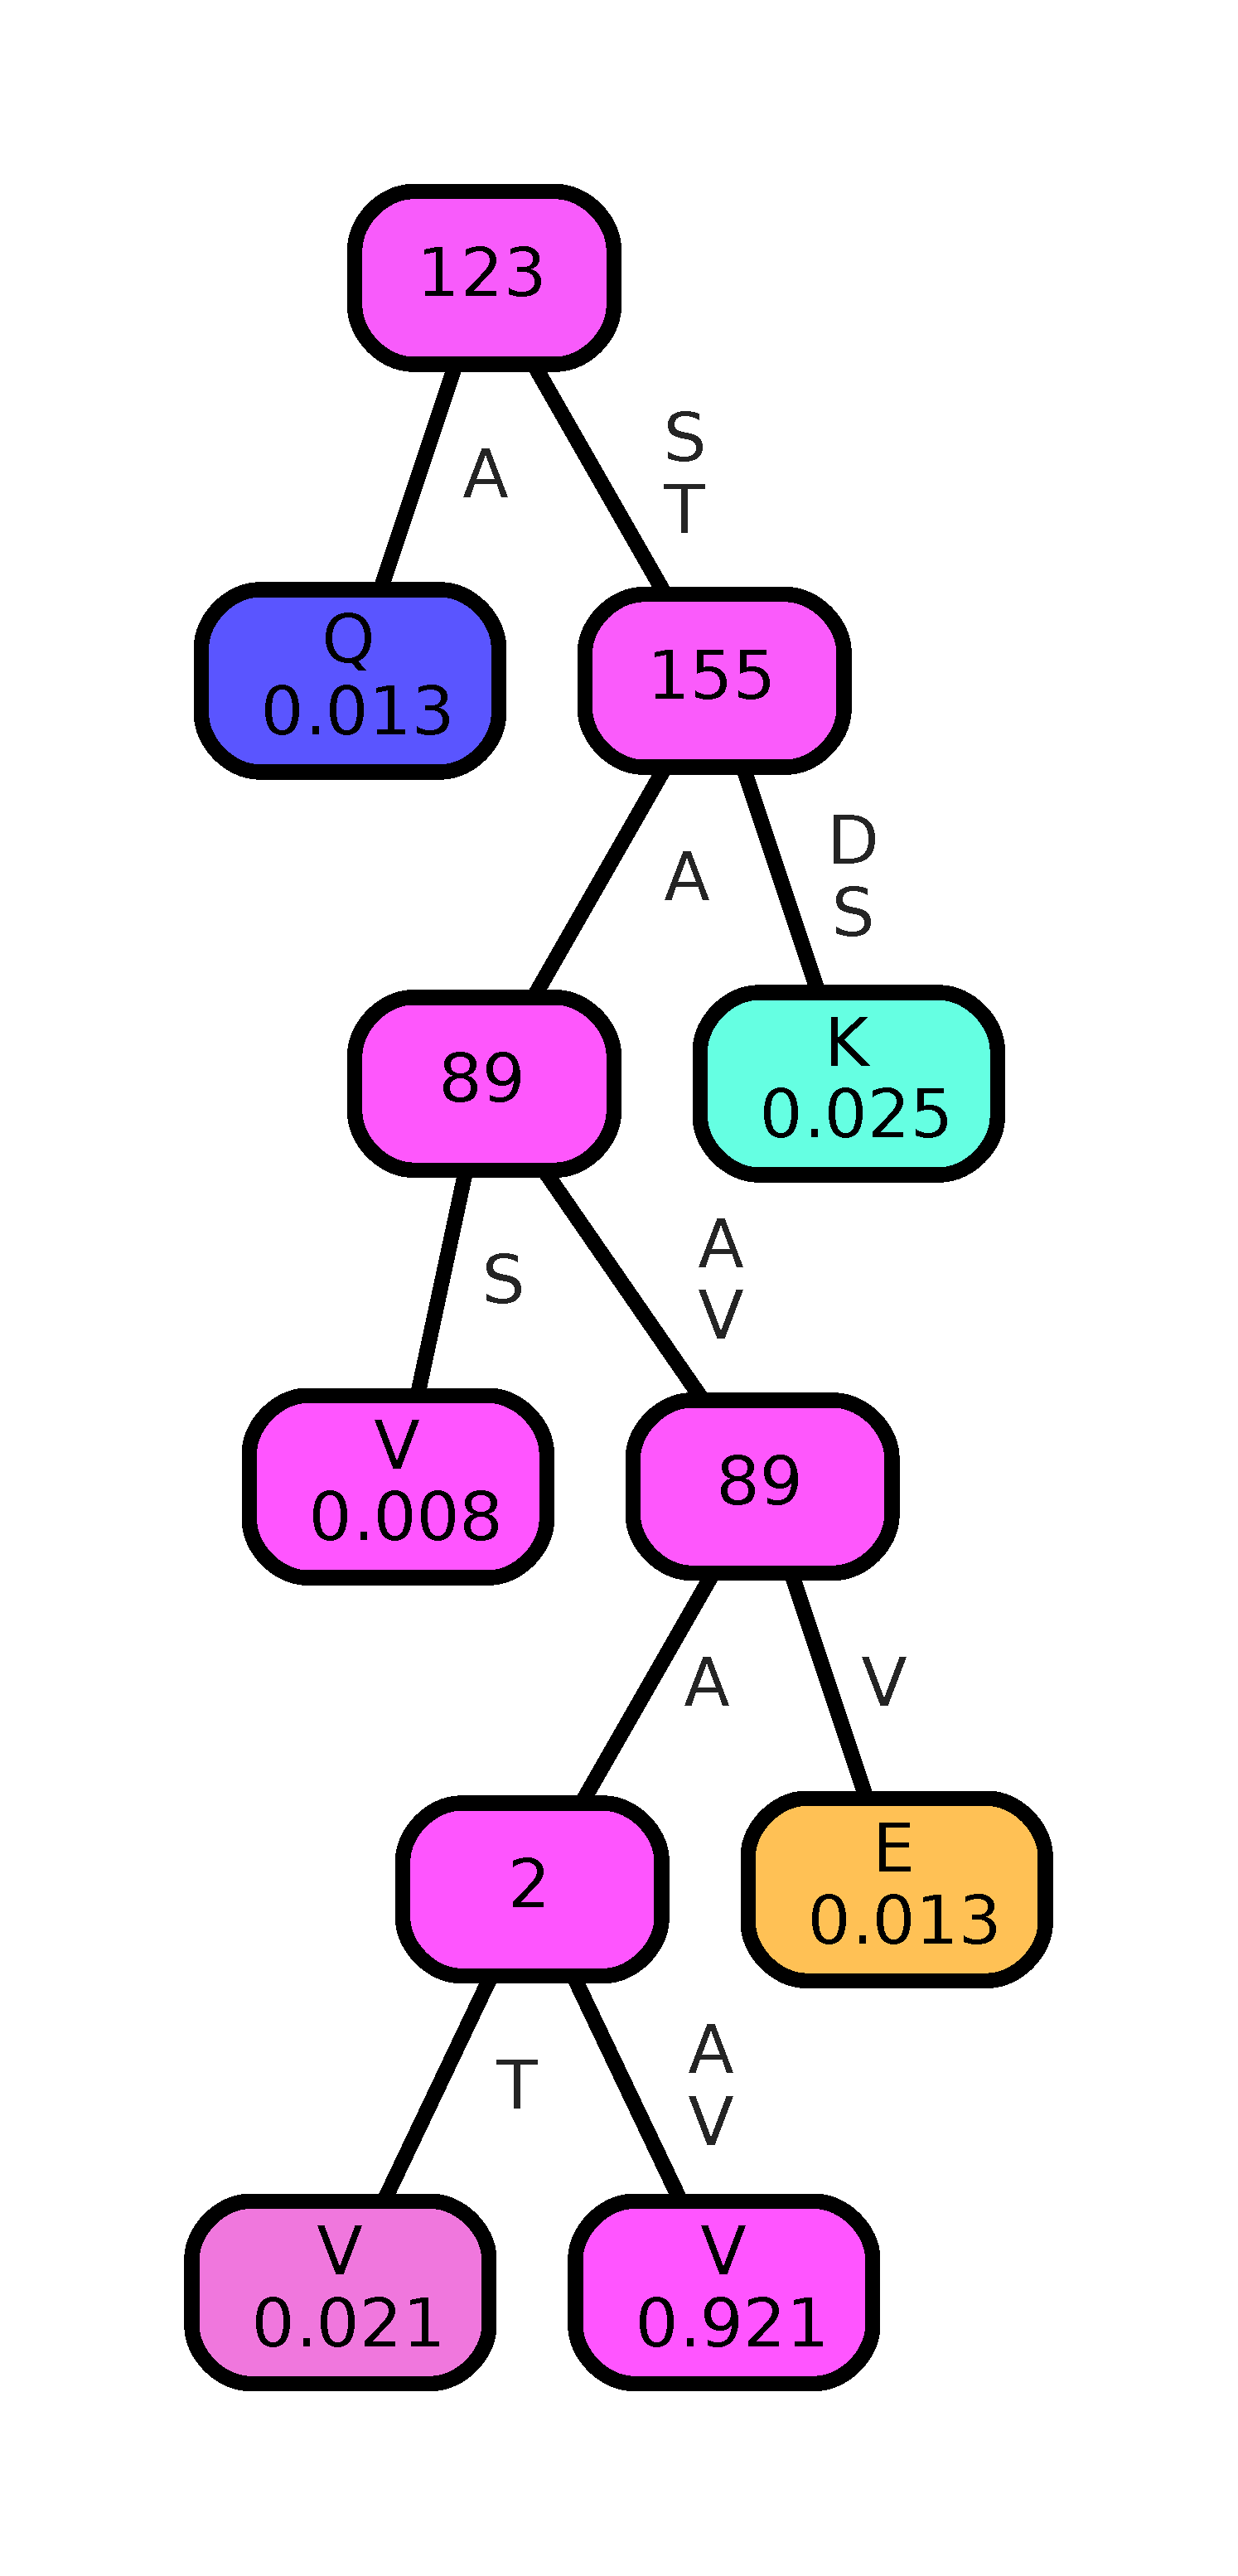
\includegraphics[width=\WDTB]{../qnet_predictions/qnet_models/trees/proc63}}; 

      
      \node[anchor=north,xcirc,inner sep=-20pt,label={[xshift=-.6in,yshift=.7in,align=center,\LCOL]-90:index\\155}] (P155) at (Z) {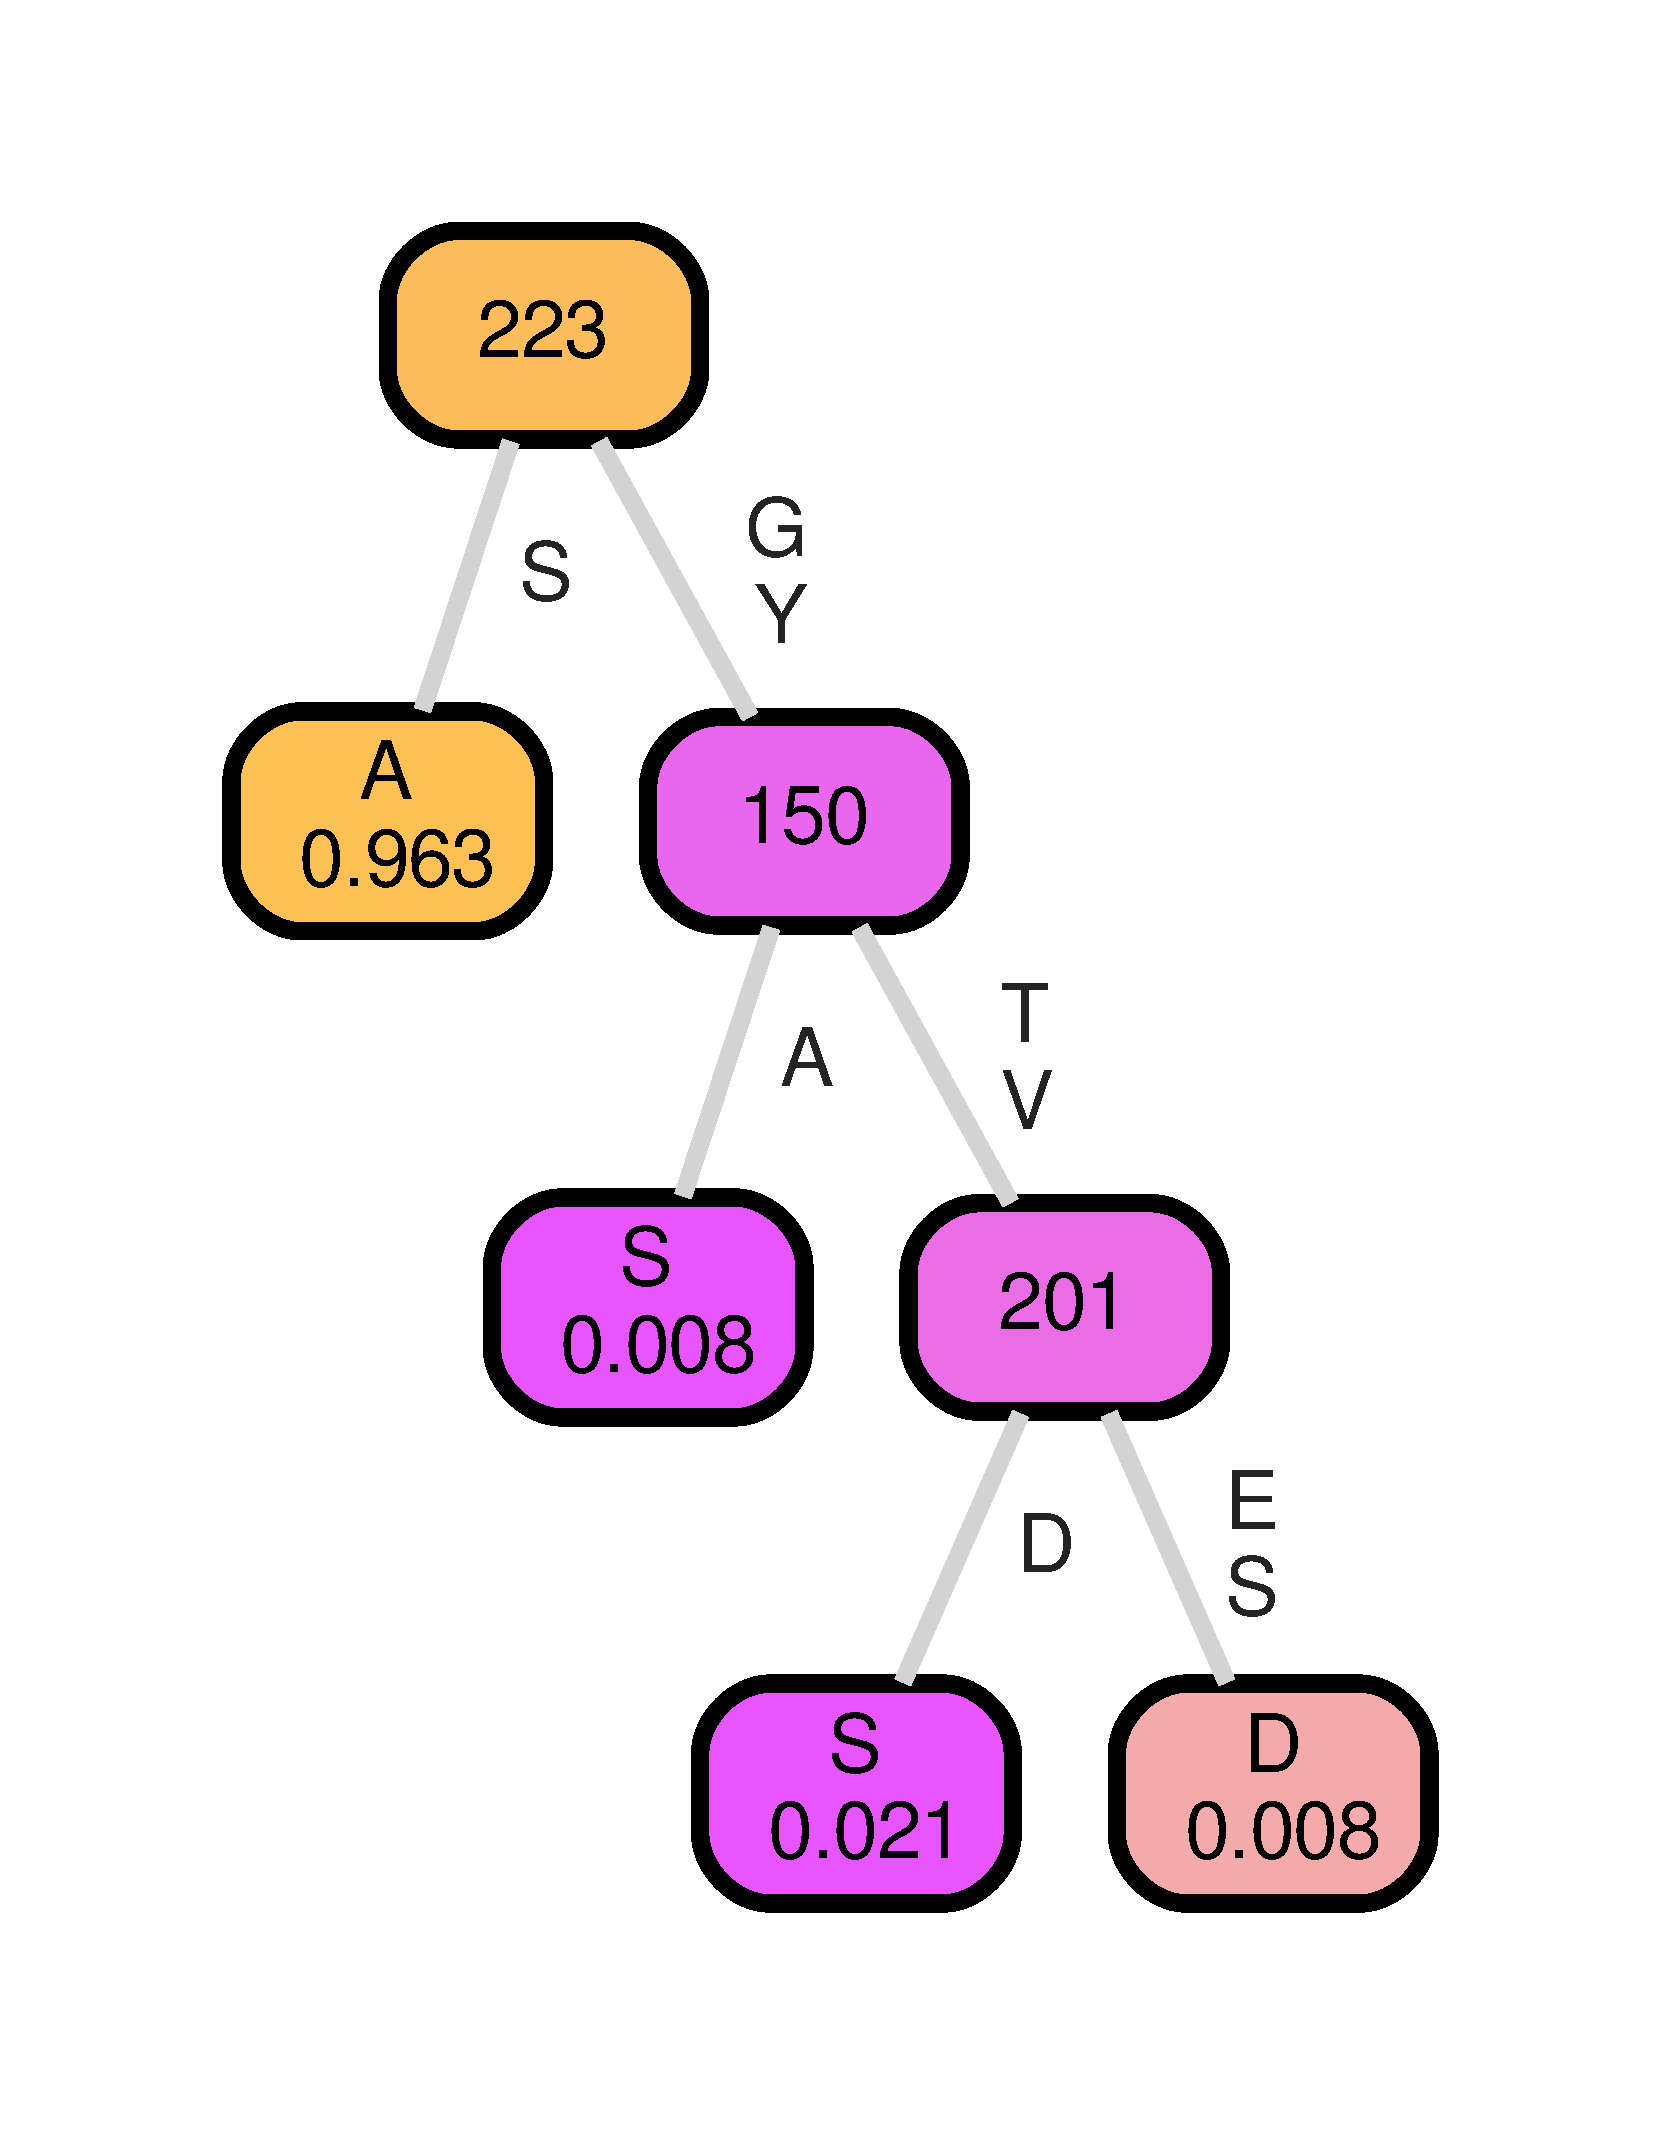
\includegraphics[width=\WDTC]{../qnet_predictions/qnet_models/trees/proc155}};

      \node[anchor=north,xcirc,inner sep=-25pt,label={[yshift=.65in,xshift=-.45in,align=center,\LCOL]-90:index\\14}] (P14) at ([xshift=-2.2in,yshift=-0.8in]P155.south) {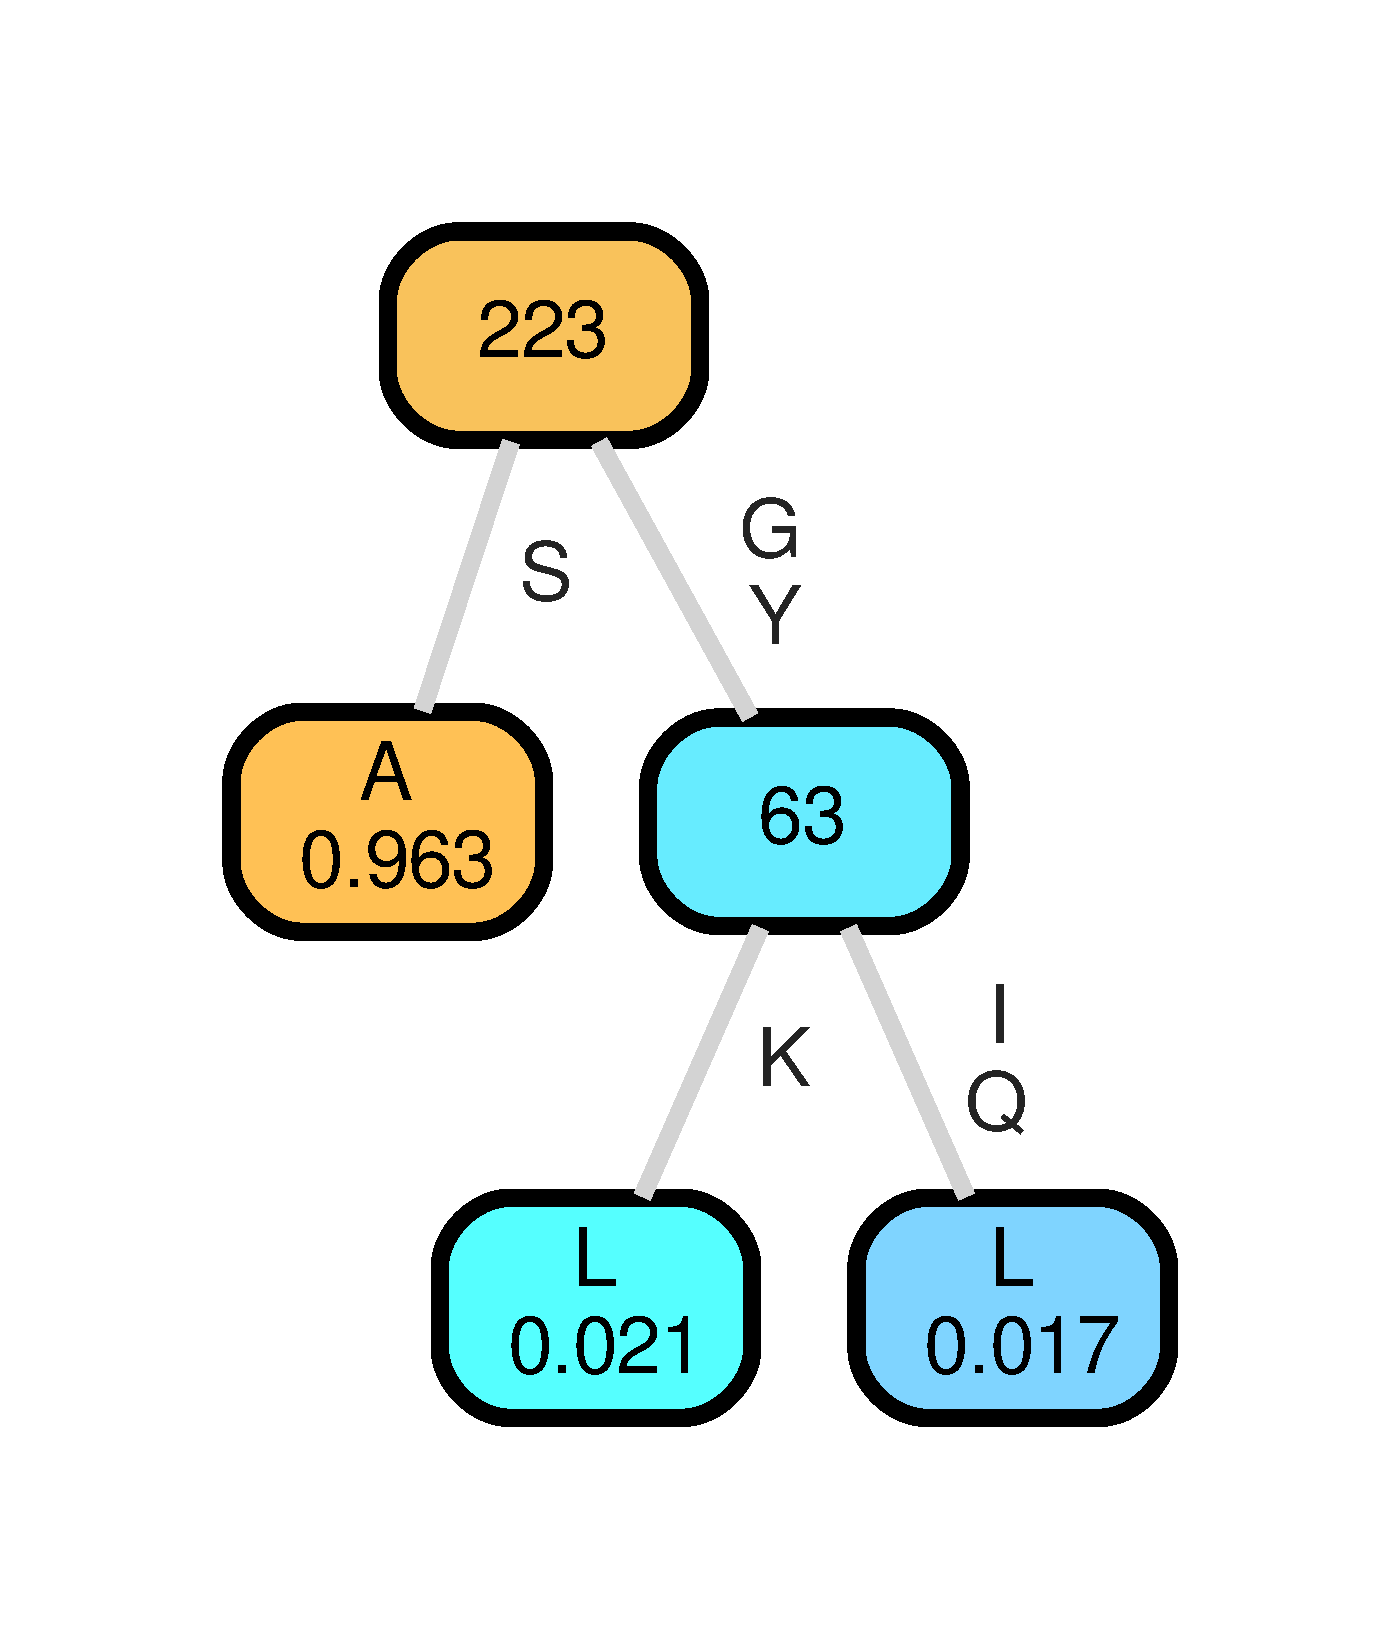
\includegraphics[width=\WDTB]{../qnet_predictions/qnet_models/trees/proc14}}; 
      
      \node[anchor=north,xcirc,inner sep=-25pt,label={[yshift=.6in,xshift=-.5in,align=center,\LCOL]-90:index\\223}] (P223) at ([xshift=-0in,yshift=-0.10in]P155.south) {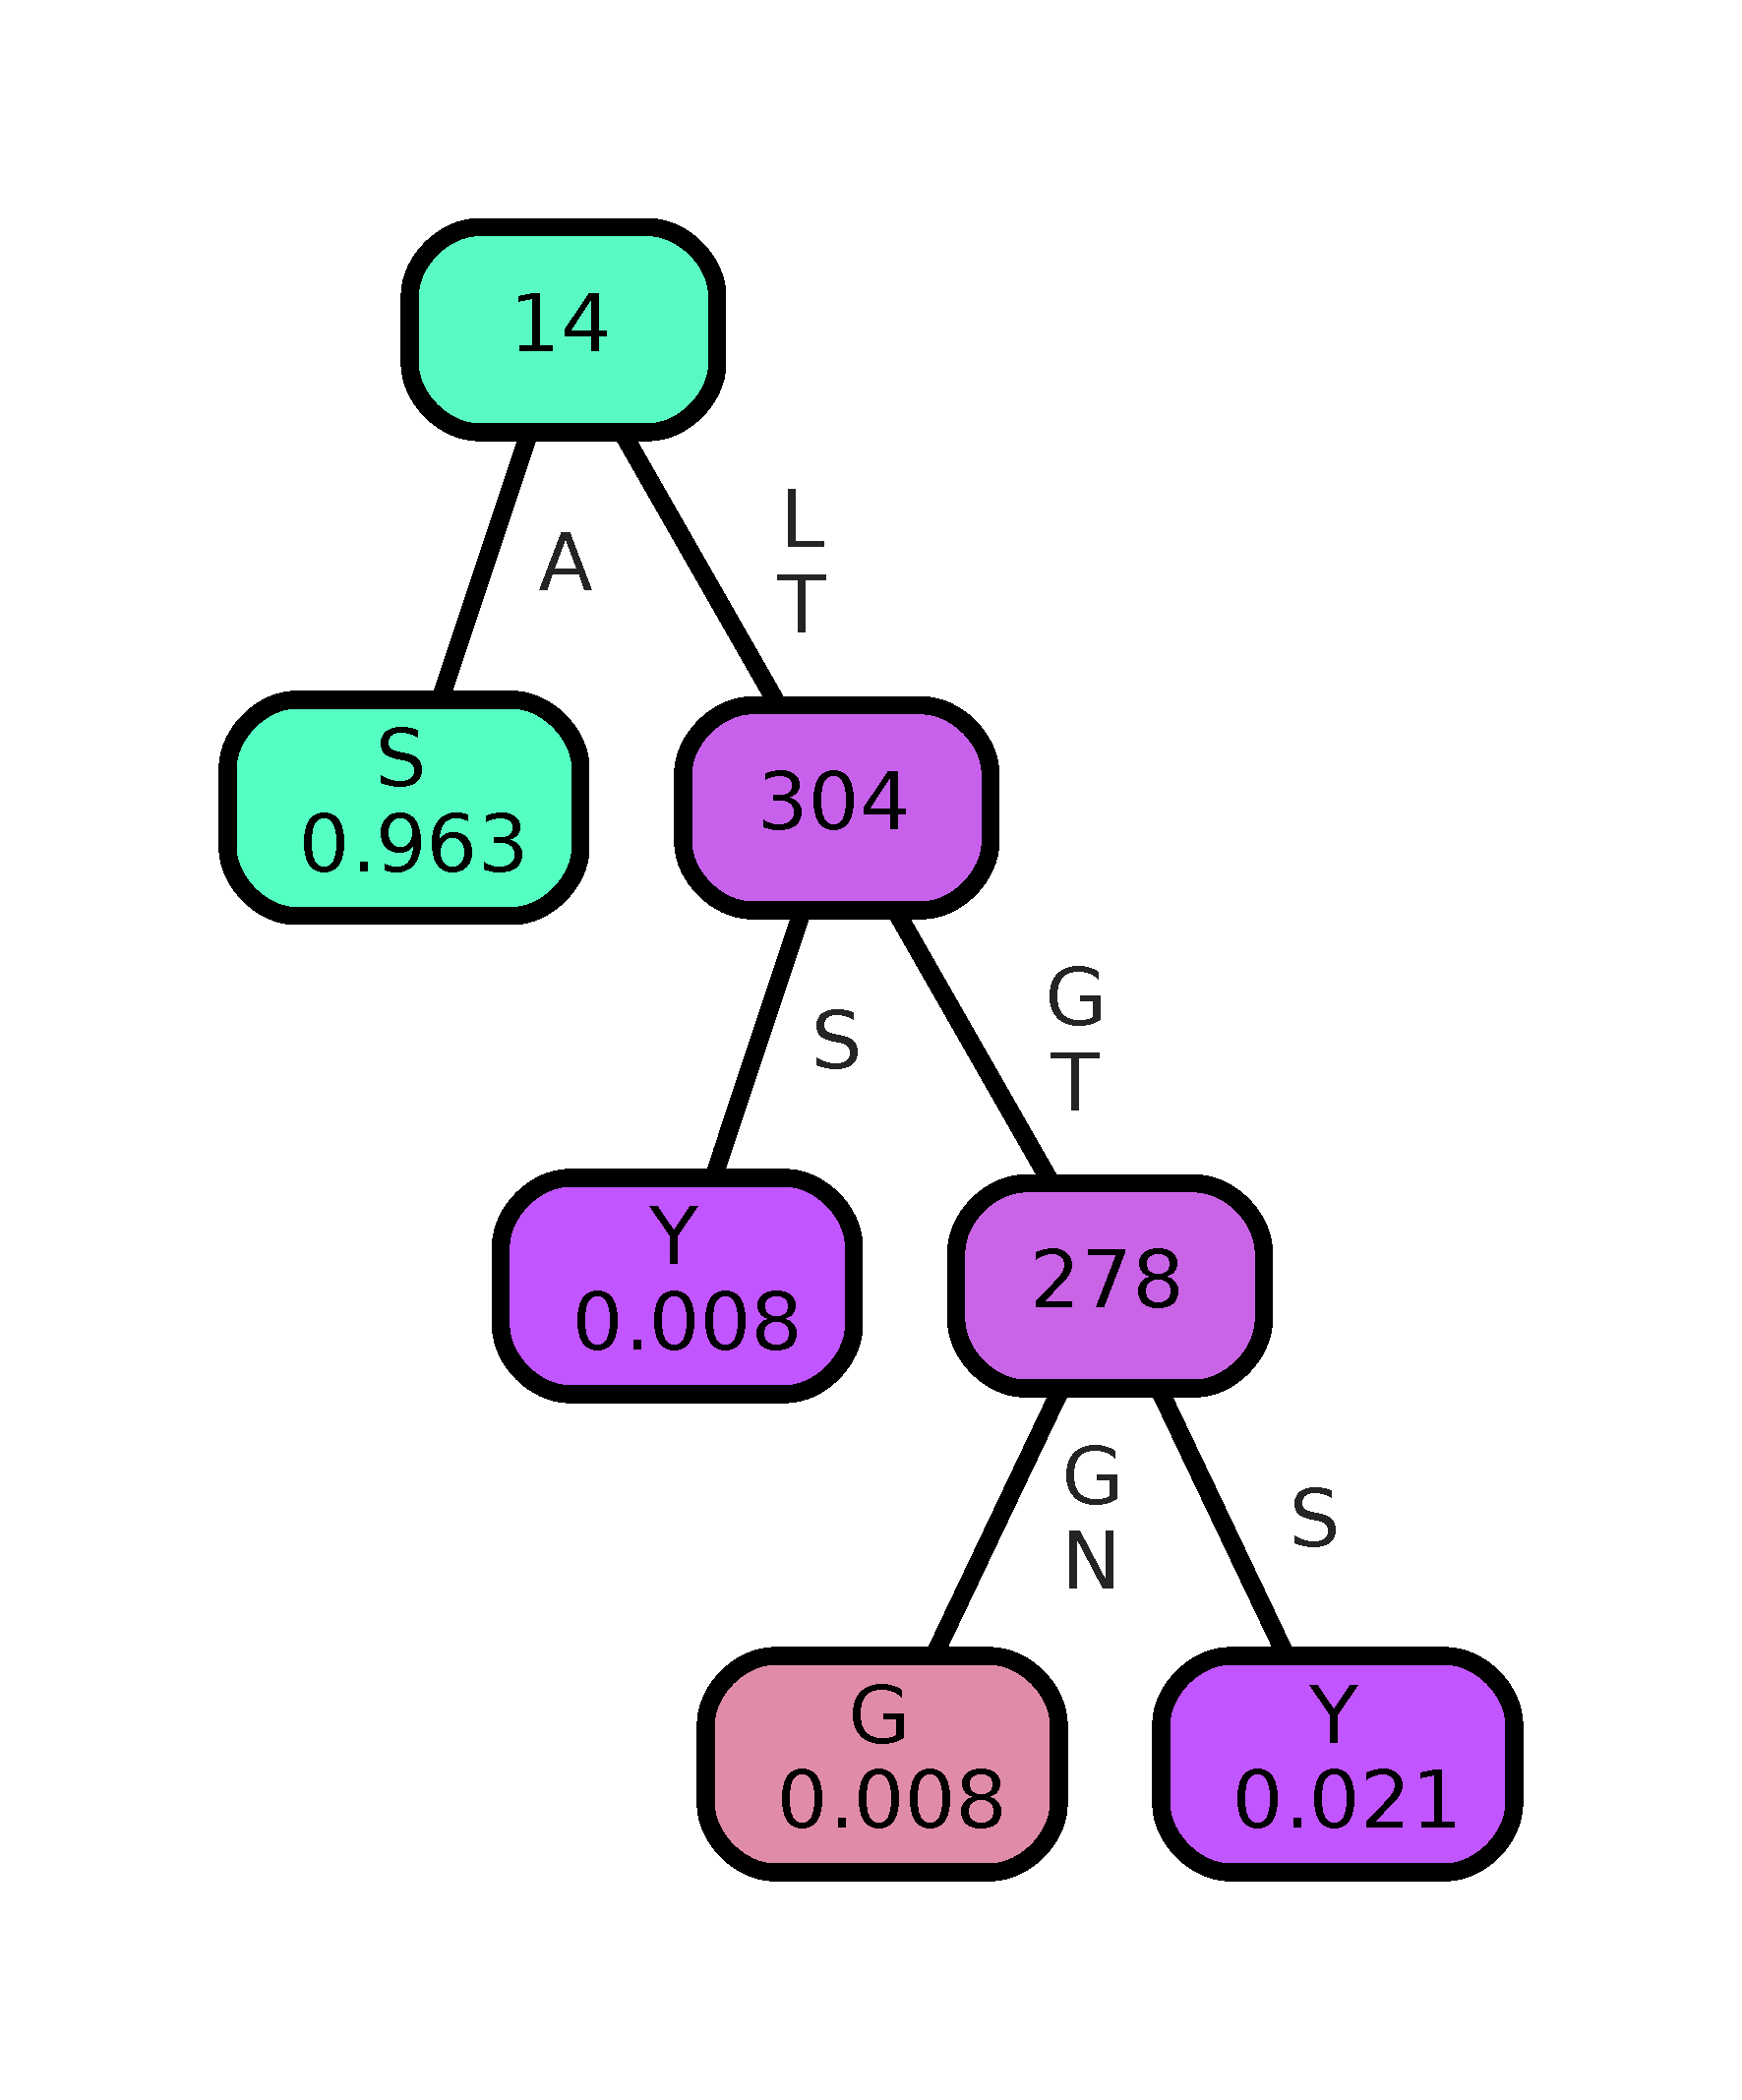
\includegraphics[width=\WDT]{../qnet_predictions/qnet_models/trees/proc223}};


      \node[text width=.13in,  rounded corners=8pt, line width=2pt,,inner sep=10pt,opacity=1,draw=\DCOLx] (X1) at ([yshift=.835in,xshift=.12in]P63) {};
      \draw [line width=\LWT,\DCOLx,-latex,] (X1)  to [out=75,in=140,looseness=1.55]  (P155);

      \node[text width=.13in,  rounded corners=8pt, line width=2pt,inner sep=10pt,opacity=1,draw=\DCOLx] (X2) at ([yshift=.845in,xshift=-.335in]P155) {};
      \draw [line width=\LWT,\DCOLx,-latex,] (X2)  to [out=0,in=60,looseness=1]  (P223);

      \node[text width=.13in,  rounded corners=8pt, line width=2pt,,inner sep=10pt,opacity=1,draw=\DCOLx] (X3) at ([yshift=.0in,xshift=.12in]P14) {};
      \draw [line width=\LWT,\DCOLx,-latex,] (X3)  to [out=150,in=-120,looseness=1.1]  (P63);

      \node[text width=.15in,  rounded corners=8pt, line width=2pt,inner sep=10pt,opacity=1,draw=\DCOLx] (X4) at ([yshift=.88in,xshift=-.34in]P223) {};
      \draw [line width=\LWT,\DCOLx,-latex,] (X4)  to [out=210,in=35,looseness=1.2]  (P14);

      \node[anchor=north,align=left,font=\bf\tt\footnotesize] (N3) at ([yshift=-6.1in,xshift=-1.85in]Z.south) {\bf\sffamily\fontsize{7}{8}\selectfont H1N1 2020-2021\\\bf\sffamily\fontsize{7}{8}\selectfont Haemagglutinin Sequences\\$\cdots$GTSRY{\color{Red1}S}KKFKPEIATRPKVRDQEGR$\cdots$\\$\cdots$GTSKY{\color{Red1}G}KKFMPEIARRPKVRNQEGR$\cdots$\\
        $\cdots$GSSKY{\color{Red1}Y}KRFTPEIVARPKVREQAGR$\cdots$\\
 $\cdots$GSSKY{\color{Red1}Y}KRFTPEIVARPKVREQAGR$\cdots$};

%A/Niger/8327/2020 
%
%A/Parana/10835/2021
%A/Gansu-Xifeng/1143/2021
%A/Sichuan/01208/2021

   \node[anchor=west,align=left,font=\bf\sffamily\fontsize{8}{10}\selectfont] (N4) at ([xshift=0.1in,yshift=.05in]N3.east) {A/Niger/8327/2020 \\
    A/Parana/10835/2021\\
      A/Gansu-Xifeng/1143/2021\\  
      A/Sichuan/01208/2021};

       \draw [ultra thick] ([yshift=.25in,xshift=.01in]N4.west) --++ (-.13in,-.190in);
       \draw [ultra thick] ([yshift=.1in,xshift=.01in]N4.west) --++ (-.13in,-.2in);
       \draw [ultra thick] ([yshift=-0.05in,xshift=.01in]N4.west) --++ (-.13in,-.2in);
       \draw [ultra thick] ([yshift=-.2in,xshift=.01in]N4.west) --++ (-.13in,-.2in);

       \node [align=center,text=IndianRed2,anchor=north] at ([xshift=-2.25in,yshift=-.1in]N4.south) {index 223};

      \node[anchor=west,rounded corners=3pt,align=center] (I1) at ([yshift=-.6in,xshift=.3in]P14.south west) {Color key (mixed colors represent distributions)};


      \definecolor{Acol}{RGB}{255,193,85}
      \definecolor{Dcol}{RGB}{255,255,85}
      \definecolor{Ecol}{RGB}{255,255,85}
      \definecolor{Gcol}{RGB}{136,255,85}
      \definecolor{Icol}{RGB}{85,255,150}
      \definecolor{Kcol}{RGB}{85,255,255}
      \definecolor{Lcol}{RGB}{85,255,255}
      \definecolor{Qcol}{RGB}{111,85,255}
      \definecolor{Scol}{RGB}{231,85,255}
      \definecolor{Tcol}{RGB}{255,85,255}
      \definecolor{Vcol}{RGB}{255,85,255}
      \definecolor{Ycol}{RGB}{255,85,97}
      
      \node[font=\bf\sffamily,anchor=north,rounded corners=3pt,text width=.1in,text height=.1in,fill=Acol,align=center,opacity=\OPC] (I1) at ([yshift=-.05in]I1.south west) {A};
      \node[font=\bf\sffamily,anchor=west,rounded corners=3pt,text width=.1in,text height=.1in,fill=Dcol,align=center,opacity=\OPC] (I1) at ([xshift=.05in]I1.east) {D};
      \node[font=\bf\sffamily,anchor=west,rounded corners=3pt,text width=.1in,text height=.1in,fill=Ecol,align=center,opacity=\OPC] (I1) at ([xshift=.05in]I1.east) {E};
      \node[font=\bf\sffamily,anchor=west,rounded corners=3pt,text width=.1in,text height=.1in,fill=Gcol,align=center,opacity=\OPC] (I1) at ([xshift=.05in]I1.east) {G};
      \node[font=\bf\sffamily,anchor=west,rounded corners=3pt,text width=.1in,text height=.1in,fill=Icol,align=center,opacity=\OPC] (I1) at ([xshift=.05in]I1.east) {I};
      \node[font=\bf\sffamily,anchor=west,rounded corners=3pt,text width=.1in,text height=.1in,fill=Kcol,align=center,opacity=\OPC] (I1) at ([xshift=.05in]I1.east) {K};
      \node[font=\bf\sffamily,anchor=west,rounded corners=3pt,text width=.1in,text height=.1in,fill=Lcol,align=center,opacity=\OPC] (I1) at ([xshift=.05in]I1.east) {L};
      \node[font=\bf\sffamily,anchor=west,rounded corners=3pt,text width=.1in,text height=.1in,fill=Qcol,align=center,opacity=\OPC] (I1) at ([xshift=.05in]I1.east) {Q};
      \node[font=\bf\sffamily,anchor=west,rounded corners=3pt,text width=.1in,text height=.1in,fill=Scol,align=center,opacity=\OPC] (I1) at ([xshift=.05in]I1.east) {S};
      \node[font=\bf\sffamily,anchor=west,rounded corners=3pt,text width=.1in,text height=.1in,fill=Tcol,align=center,opacity=\OPC] (I1) at ([xshift=.05in]I1.east) {T};
      \node[font=\bf\sffamily,anchor=west,rounded corners=3pt,text width=.1in,text height=.1in,fill=Vcol,align=center,opacity=\OPC] (I1) at ([xshift=.05in]I1.east) {V};
      \node[font=\bf\sffamily,anchor=west,rounded corners=3pt,text width=.1in,text height=.1in,fill=Ycol,align=center,opacity=\OPC] (I1) at ([xshift=.05in]I1.east) {Y};

      % \node[font=\bf\sffamily,anchor=north,rounded corners=3pt,text width=.1in,text height=.1in,fill=DarkOrange3!70,align=center,opacity=\OPC] (I1) at ([yshift=-.05in]I1.south) {A};

      % \node[font=\bf\sffamily,anchor=north,rounded corners=3pt,text width=.1in,text height=.1in,fill=SeaGreen2,align=center,opacity=\OPC] (I1) at ([yshift=-.05in]I1.south) {C};

      % \node[font=\bf\sffamily,anchor=north,rounded corners=3pt,text width=.1in,text height=.1in,fill=DodgerBlue2!80,align=center,opacity=\OPC] (I1) at ([yshift=-.050in]I1.south) {G};
    \end{tikzpicture}
  };

  \node [anchor=south west] (L1) at ([yshift=-.2650in]T.north west) {\Large a.};
  \node [anchor=south west] (L2) at ([yshift=-3.25in]T.north west) {\Large c.};
  \node [anchor=south west] (L3) at ([yshift=-5.65in]T.north west) {\Large d.};

\end{tikzpicture}

   \else
   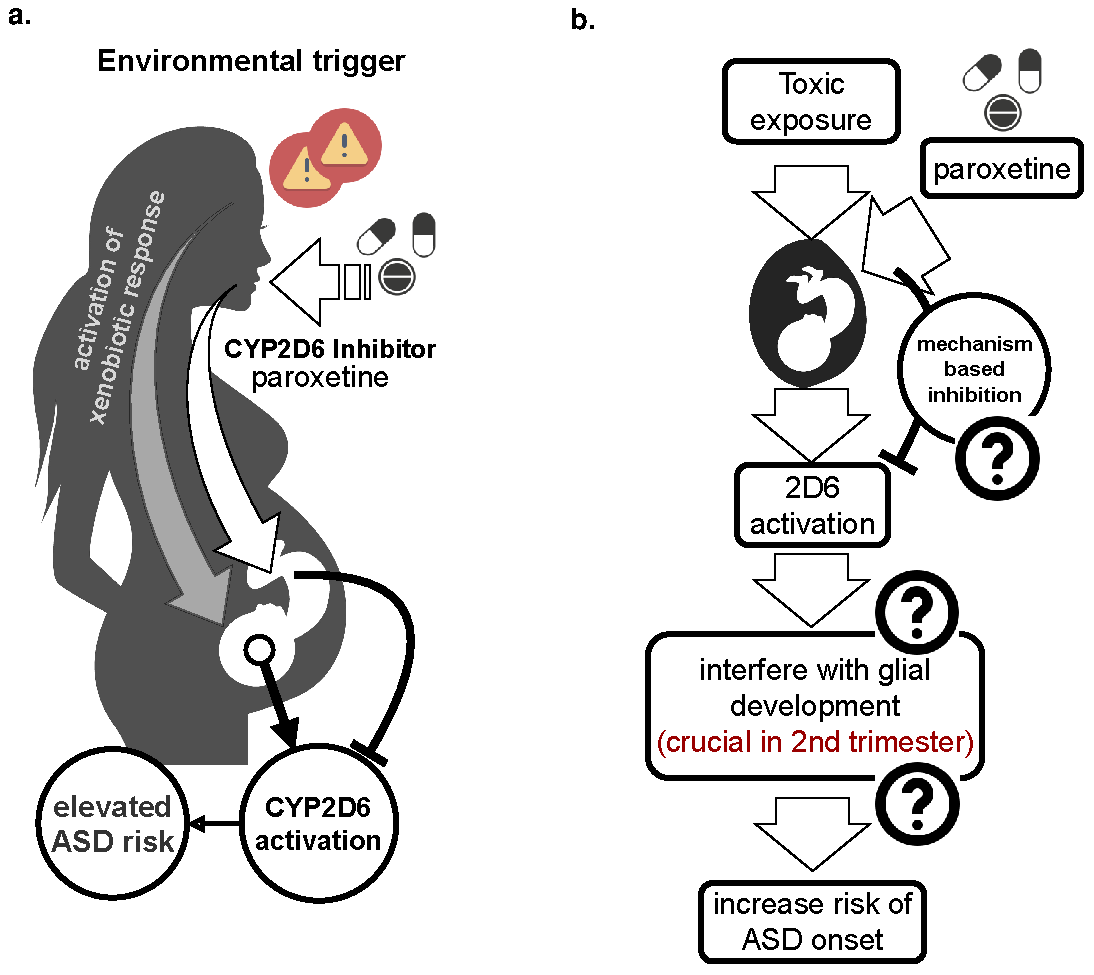
\includegraphics[width=\textwidth]{Figures/External/scheme}
  \fi
 
%\includegraphics[width=\textwidth]{Figures/asdgenescheme}
\captionN{}\label{figscheme}
\end{figure}


\bibliographystyle{naturemag}
\bibliography{asdgene,mergedbib}


\end{document}


(i.e., SSC, Simons Searchlight, SPARK, AIC) being requested in this application? If Yes, please include description of the request and use below.